\begin{appendices}

%
\chapter{Test Plan}
\label{ref:testplan}
\small
\begin{longtable}{| p{2cm} | p{0.5cm} | p{4cm} | p{5cm} | p{3cm} |}
	\hline
		%HEADER
		\bf{Section} & \bf{Test No} & \bf{Test Name} & \bf{Description} & \bf{Expected} \\ \hline
		
		%--- UDP CLIENT
		\bf{UDP Client}&&&& \\ \hline
		
		% Business Logic
		Logic &&&& \\ \hline
		&& TestStartUp() & Creates a client object before each test & n/a\\ \hline
		&& TestCleanUp() & No clean-up needed & n/a \\ \hline
		&1& Connect-Disconnect() & The client connects performs no action then disconnects & n/a \\ \hline
		&2& CreateClientObj() & A client object is created & n/a \\ \hline
		&3& SendPacket() & Sends a single UDP packet & n/a\\ \hline
		&4& CheckGridSend() & Checks the method sends out the correct number this depends on grid size & n/a \\ \hline
		
		% UI
		UI &&&& \\ \hline
		&& TestStartUp() & Loads up a fresh window from the command line & n/a \\ \hline
		&& TestCleanUp() & Clicks the X in the top right corner & n/a \\ \hline
		&5& ConnectClick() & Clicks the "Connect" button & n/a \\ \hline
		&6& RestartClick() & Clicks the "Connect" button then the "Restart" button & n/a \\ \hline
		&7& Connect-InvertCheck() & Clicks the "Connect" button and checks all the buttons invert their "Enabled" property correctly & Connect(Disabled), Restart(Enabled) \\\hline
		&8& Restart-InvertCheck() & Clicks the "Connect" button, then the "Reset" button and checks the "Enabled" properties for all buttons are correct & Connect(Enabled), Restart(Disabled) \\\hline
		&9& TextEntry() & Enters text into the text box and then "Connect" is clicked & n/a \\ \hline
				
		%--- UDP SERVER
		\bf{UDP Server} &&&& \\ \hline		
		
		%Business 
		Logic &&&& \\ \hline
		&& TestStartUp() & Creates the client object & n/a \\ \hline
		&& TestCleanUp() & n/a & n/a  \\ \hline
		&10& CreateObject() & Tests that the server object can be created successfully & n/a \\ \hline
		&11& WaitForTimeout() & Starts the server and checks it closes cleanly after time-out & n/a \\ \hline
		
		% UI
		UI &&&& \\ \hline
		&& TestStartUp() & Loads up a fresh window from the CMD line & n/a \\ \hline
		&& TestCleanUp() & Clicks the X in the top right hand corner & n/a  \\ \hline
		&12& StartClick() & Click the "Start" button & n/a \\ \hline
		&13& RandomiseClick() & Click the "Randomise" button & n/a \\ \hline
		&14& Start-ResetClick() & Clicks the "Start" button then resets and checks it returns to it's default state & n/a \\ \hline
		&15& Randomise-ResetClick() & Clicks the "Randomise" button, the resets and checks it returns to it's default state & n/a \\ \hline
		&16& Start-CheckInvert() & "Start" button clicked and then the test checks for "Enabled" property is inverted & n/a \\ \hline
		&17& RestartCheckInvert() & "Start" then "Restart" button clicked and the test then checks for the correct inverting of the buttons "Enabled" property Start = Enabled, Restart = Disabled & n/a \\ \hline
		&18& Stat-PacketLossReset() & Checks when the restart button is clicked the statistics is returned to default & "-" \\ \hline
		&19& Stat-TotalPacketLossReset() & Checks when the restart button is clicked the statistics is returned to default & "-" \\ \hline
		&20& Stat-TotalPacketSentReset() & Checks when the restart button is clicked the statistics is returned to default & "-" \\ \hline
		&21& Stat-CheckDeafult() & "Start" is clicked and the test then waits for a time-out, it then checks the default values of the statistics & PacketLoss(100) \\ \hline
		
		%--- UDP COMBINED		
		Live Tests &&&& \\ \hline
		&& TestStartUp() & Both windows were opened on the command line & n/a \\ \hline
		&& TestCleanUp() & Both windows are closed by automated actions & n/a \\ \hline
		&22& SendAndRecieve-Valid() & The client sends packages to the server and the server accepts packets & n/a \\ \hline
		&23& SendAndRecive-Valid-Twice() & The performs the same action at the above test but does the whole loop an extra time to check if the reset works correctly & n/a \\ \hline
		&24& SendAndRecieve-Invalid() & This test doesn't connect the client to the server but a random IP on the network, this is to check the server will act accordingly & n/a \\ \hline

		\bf{FTP Server} &&&& \\ \hline
		
		%--- FTP Logic
		Logic &&&& \\ \hline
		&& TestStartUp() & Creates the server object & n/a \\ \hline
		&& TestCleanUp() & n/a & n/a \\ \hline
		&25& CreateObject() & Creates a version of the server object & n/a \\ \hline
		&26& ServerSetup() & Performs the server set-up & n/a \\ \hline
		&27& ServerStart() & Sets up the server and starts it & n/a \\ \hline
		&28& ServerStartStop() & Does a fully cycle for the server & n/a \\ \hline
		
		%--- FTP Combined
		&& TestStartUp() & Loads up FTP Server and FileZilla & n/a \\ \hline
		&& TestCleanUp() & Closes each window with automated actions & n/a \\ \hline
		&& ValidConnection() & Automated UI test that simulates a valid connection and checks elements on the UI for signs of a valid connection & n/a \\ \hline
		&& InvalidConnection() & Test that attempts to connect to a non working server & n/a \\ \hline
		&& DownloadFile() & A test that simulates a download of a file and checks it completes fully & n/a \\ \hline
		&& InteruptDownload() & Test that starts a download and interrupts it before completion & n/a \\ \hline
	\hline
\end{longtable}

Packet Script Test Plan for the default effects.

\begin{longtable}{| p{2cm} | p{0.5cm} | p{4cm} | p{5cm} | p{3cm} |}
	\hline	
	\bf{Section} & \bf{Test No} & \bf{Test Name} & \bf{Description} & \bf{Expected} \\ \hline
	\bf{Effects} &&&& \\ \hline
	PacketLoss &&&& \\ \hline
	&1& StartPacketLoss() & Starts the script with the expected parameter (e.g. -pl 10) &  Script should start PacketLoss mode \\ \hline
	&2& PacketLossEffect() & Pings the script and checks the effect on the ping packets, the test pings until one packet is lost. Checking for exact percentages isn't reliable enough & Some packet loss \\ \hline	
	Latency &&&& \\ \hline
	&3& StartLatency() & Starts the script with valid parameters for latency (e.g. -l 10) & Script should start in Latency mode \\ \hline
	&4& LatencyEffect() & Pings the script and checks the latency value within a margin of error & Latency effect on ping packets \\ \hline	
	Bandwidth &&&& \\\hline
	&5& StartBandwidth() &  Starts the script with the expected parameters (e.g. -rl 100) & Script should start in Bandwidth limit mode \\ \hline
	&6& BandwidthEffect() & Starts bandwidth mode and starts pinging the localhost, after a certain amount of packets the rate is calculated and checked against the rate limit value & n/a \\\hline
	Script &&&& \\ \hline
	&7& LatencyValidation() & Check that the validation works for the latency mode & Range = 1-1000ms \\\hline
	&8& PacketLossValidation() & Check that the validation works for the packet loss mode & Range = 1-100\%\\\hline
	&9& BandwidthValidation() & Checks that validation works for bandwidth mode & Range =  1-10000B/s\\\hline
	
\end{longtable}

\begin{center}
\chapter{HTTP Testing}
\label{ref:httpTesting}
\end{center}


\begin{tabular}{| l | l |}
	\hline
	{\bf Effect Value (m/s)} & {\bf Page Load Time (Seconds)} \\\hline
	50					& 0.952430844306946	 \\\hline
    100					& 1.67083732287089 \\\hline
	150 				& 2.4343535900116 \\\hline
	200					& 3.2439550558726 \\\hline
	250					& 3.91064143180847\\\hline
	300 				& 4.64833283424377\\\hline
	350					& 5.55461764335632\\\hline
	400					& 6.32855240503947\\\hline
	450					& 7.27884976069133\\\hline
	500					& 7.88651315371196\\\hline
	550					& 9.28576032320658\\\hline
	600					& 10.0889756679535\\\hline
	650					& 10.9339879353841\\\hline
	700					& 11.7680953343709\\\hline
	750					& 12.5511389573415\\\hline
	800					& 12.4368558724721\\\hline
	850					& 15.2392919858297\\\hline
	900 				& 16.2793971697489\\\hline
	950					& 20.7436565558116\\\hline
	1000				& 19.1623089313507\\\hline
\end{tabular}
\begin{figure}[h]
	\caption{Page loads times of \url{https://en.wikipedia.org/wiki/University_of_Hull} when latency is active}
	\label{ref:latencyHttp}
\end{figure}

\chapter{FTP Testing}
\label{ref:ftpTesting}
\begin{center}

\begin{tabular}{| l | l |}
	\hline
	{\bf Description} 	& {\bf Download Time (Minutes:Seconds)} \\\hline
	No script			& 0:15 \\\hline
	0m/s				& 0:17 \\\hline
	10 	m/s				& 0:34 \\\hline
	50 	m/s				& 0:41 \\\hline
	100 m/s				& 1:29 \\\hline
	150 m/s				& 2:02 \\\hline
	200 m/s				& 2:46 \\\hline
		
\end{tabular}
\begin{figure}[h]
		\caption{Time to download a 5MB file when latency is being simulated by the tool}
	\end{figure}	

\begin{tabular}{| l | l |}
	\hline
	{\bf Description} 	& {\bf Download Time (Minutes:Seconds)} \\\hline
	1\%					& 0:35 \\\hline
	5\%					& 0:38 \\\hline
	10\%				& 1:02 \\\hline
	15\%				& 1:45 \\\hline
	20\%				& 2:38 \\\hline
	25\%				& 4:34 \\\hline
\end{tabular}
\begin{figure}[h]
		\caption{Time to download a 5MB file when packet loss is being simulated by the tool}
\end{figure}	
\end{center}

%
\chapter{UDP Testing}
\label{ref:udpTesting}
\newcommand{\udpScale}{0.5}
\newcommand{\figureText}[1]{#1\% packet loss}

\begin{figure}[!htb]
\minipage{0.32\textwidth}
  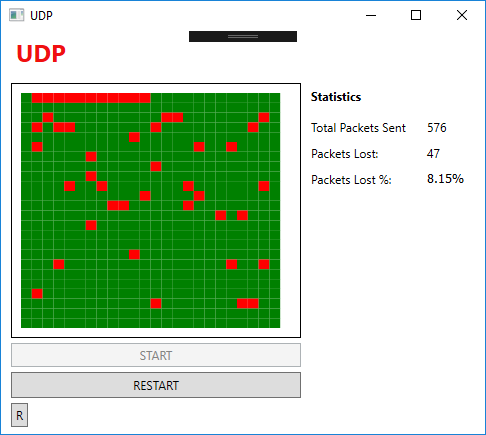
\includegraphics[width=\linewidth]{PacketLoss5}
  \caption{\figureText{5}}
\endminipage\hfill
\minipage{0.32\textwidth}
  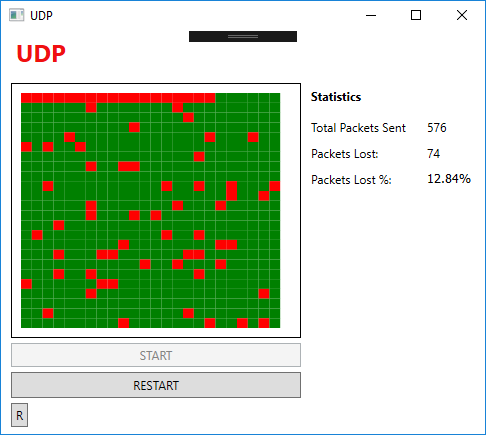
\includegraphics[width=\linewidth]{PacketLoss10}
  \caption{\figureText{10}}
\endminipage\hfill
\minipage{0.32\textwidth}
  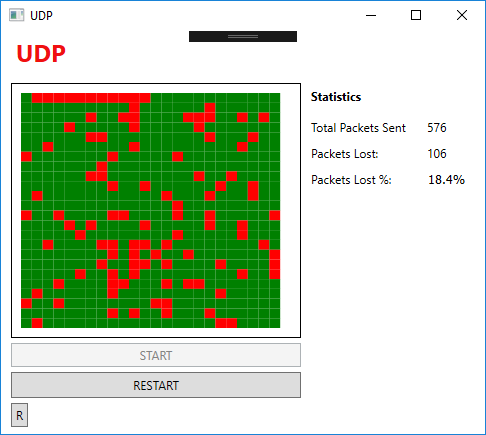
\includegraphics[width=\linewidth]{PacketLoss15}
  \caption{\figureText{15}}
\endminipage
\end{figure}

\begin{figure}[!htb]
\minipage{0.32\textwidth}
  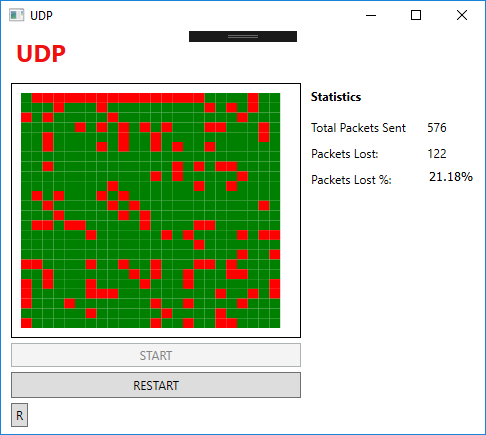
\includegraphics[width=\linewidth]{PacketLoss20}
  \caption{\figureText{20}}
\endminipage\hfill
\minipage{0.32\textwidth}
  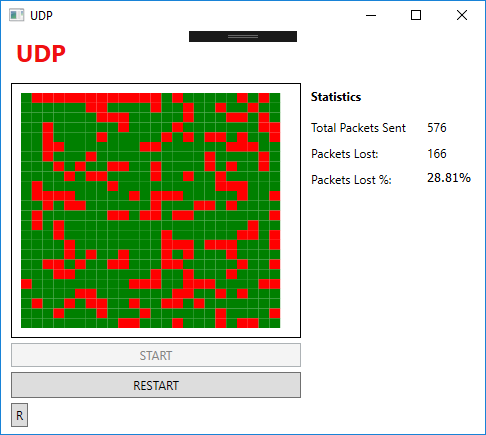
\includegraphics[width=\linewidth]{PacketLoss25}
 \caption{\figureText{25}}
\endminipage\hfill
\minipage{0.32\textwidth}
  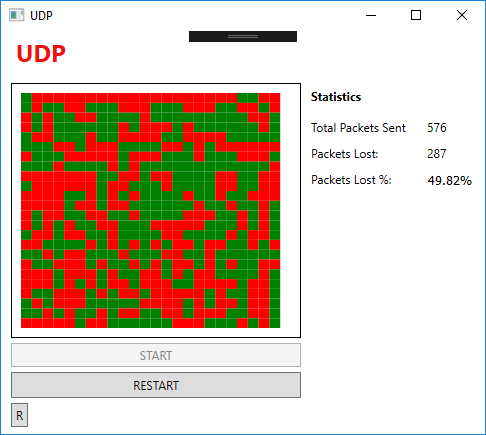
\includegraphics[width=\linewidth]{PacketLoss50}
  \caption{\figureText{50}}
\endminipage
\end{figure}

\begin{figure}[!htb]
\minipage{0.32\textwidth}
  	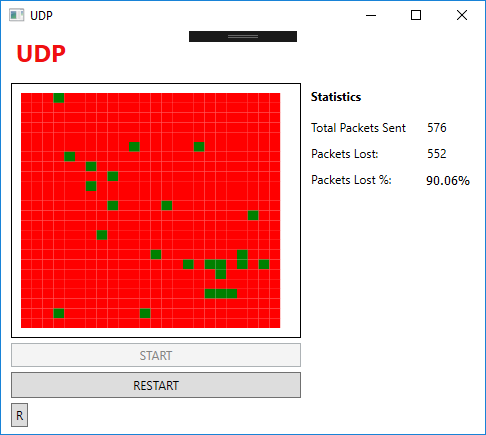
\includegraphics[width=\linewidth]{PacketLoss95}
  	\caption{\figureText{95}}
\endminipage\hfill
\minipage{0.32\textwidth}
  	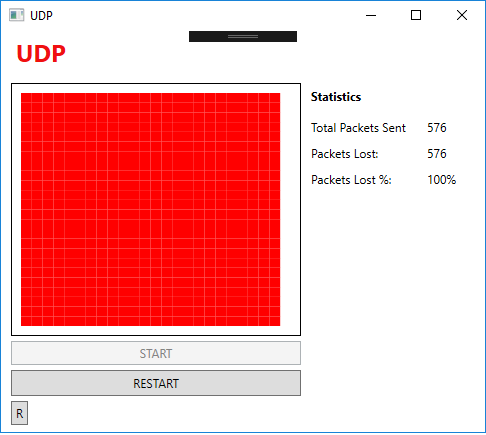
\includegraphics[width=\linewidth]{PacketLoss100}
  	\caption{\figureText{100}}
\endminipage\hfill
\minipage{0.32\textwidth}
  	\hfill
\endminipage
\end{figure}

%
\chapter{GitHub Issues}
\begin{center}
	\label{ref:GitHubAppendix}
	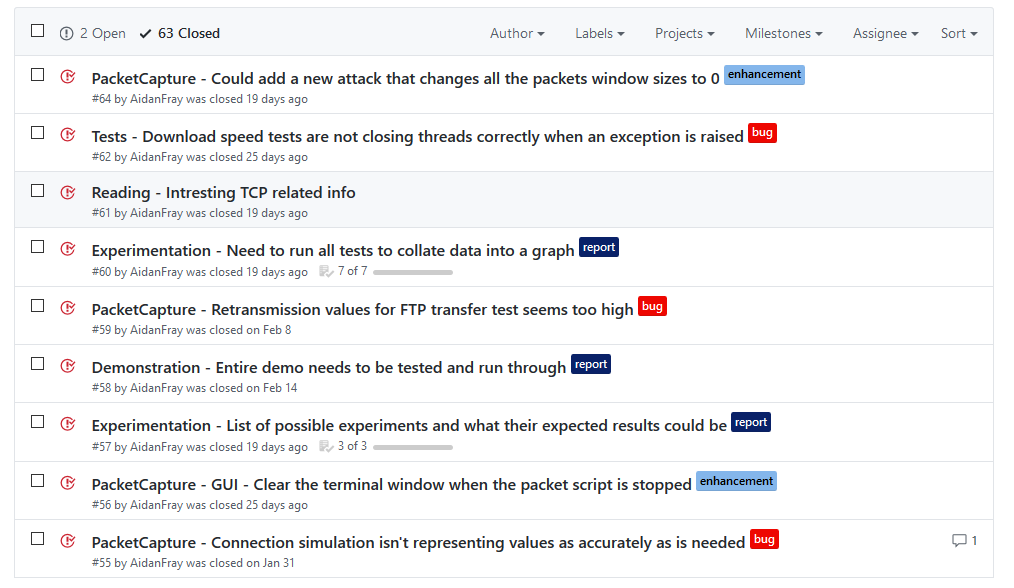
\includegraphics[scale=0.6]{github_issues}
	\begin{figure}[h]
		\caption{Snapshot of actual issues created in the project}
		\label{ref:GitHubIssues}
	\end{figure}			
\end{center}

\begin{center}
	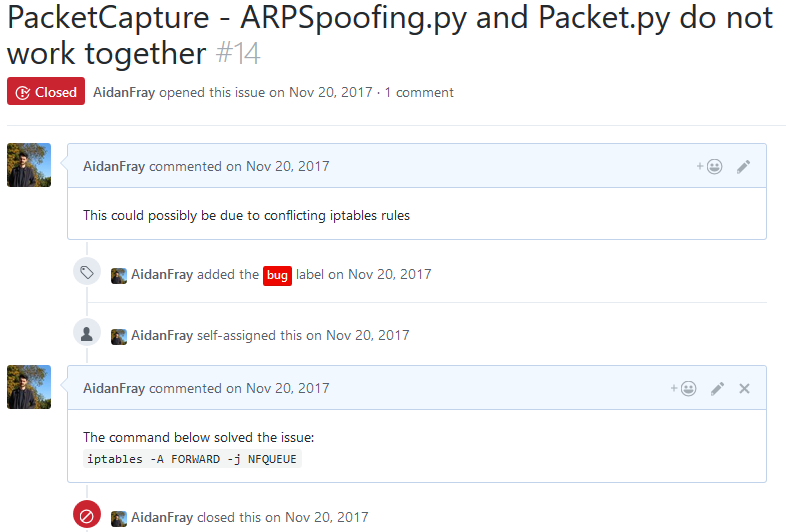
\includegraphics[scale=0.6]{github_issue_des}
	\begin{figure}[h]
		\caption{Example of an issue with discussion}
		\label{ref:GitHubIssueExample}
	\end{figure}	
\end{center}

%
\chapter{Testing Correctness}
\begin{center}
	\label{ref:testingCorrect}
	\begin{tabular}{| p{3cm} | p{5cm} | p{1cm} |}
	
	\lineend
	%--- UDP CLIENT
	\header{UDP Client}\lineend
	
	\bf{Logic} && \\ \lineend
	UC-L3	& Connect-Disconnect() 			& \Pass \\ \lineend
	UC-L4	& CreateClientObj() 			& \Pass \\ \lineend
	UC-L5	& SendPacket() 					& \Pass \\ \lineend
	UC-L6	& CheckGridSend() 				& \Pass \\ \lineend
	
	\bf{UI} && \\ \lineend	
	UC-U3 	& ConnectClick() 				& \Pass \\ \lineend
	UC-U4	& RestartClick() 				& \Pass \\ \lineend
	UC-U5	& Connect-InvertCheck() 		& \Pass \\ \lineend
	UC-U6	& Restart-InvertCheck() 		& \Pass \\ \lineend
	UC-U7	& TextEntry() 					& \Pass \\ \lineend
	
	%--- UDP Server
	\header{UDP Server}\lineend
	
	\bf{Logic} && \\ \hline
	US-L3	& CreateObject() 				& \Pass \\ \lineend
	US-L4	& WaitForTimeout() 				& \Pass \\ \lineend	
	
	\bf{UI} && \\ \lineend
	US-U3	& StartClick()					& \Pass \\ \lineend
	US-U4	& RandomiseClick() 				& \Pass \\ \lineend
	US-U5	& Start-ResetClick() 			& \Pass \\ \lineend
	US-U6	& Randomise-ResetClick()		& \Pass \\ \lineend
	US-U7	& Start-CheckInvert() 			& \Pass \\ \lineend
	US-U8	& RestartCheckInvert() 			& \Pass \\ \lineend
	US-U9	& Stat-PacketLossReset()		& \Pass \\ \lineend
	US-U10	& Stat-TotalPacketLossReset() 	& \Pass \\ \lineend
	US-U11	& Stat-TotalPacketSentReset() 	& \Pass \\ \lineend
	US-U12	& Stat-CheckDeafult()		  	& \Pass \\ \lineend
		
	\header{UDP Combined}\lineend
	\bf{Live} && \\ \lineend
	U-3		& SendAndRecieve-Valid() 		& \Pass \\ \lineend
	U-4		& SendAndRecive-Valid-Twice() 	& \Pass \\ \lineend
	U-5		& SendAndRecieve-Invalid() 		& \Pass \\ \lineend	
	
\end{tabular}

	\begin{figure}[h]
		\caption{Testing correctness for the UDP Server and Client}
		\label{ref:testingUDP}
	\end{figure}
	
	\begin{tabular}{| p{3cm} | p{5cm} | p{1cm} |}

\lineend
\header{PacketLoss}
P-1		& StartPacketLoss() 		& \Pass \\ \lineend
P-2		& PacketLossEffect()		& \Pass \\ \lineend

\header{Latency} 
L-1		& StartLatency() 			& \Pass	\\ \lineend
L-2		& LatencyEffect() 			& \Pass \\ \lineend

\header{Bandwidth} 
B-1		& StartBandwidth()			& \Pass \\ \lineend	
B-2		& BandwidthEffect() 		& \Pass \\ \lineend

\header{Out-Of-Order}
O-1		& StartOrder()				& \Pass \\ \lineend
O-2		& OutOfOrderEffect()		& \Pass \\ \lineend

\header{Jitter}
J-1		& StartJitter()			 	& \Pass \\ \lineend
J-2		& JitterEffect() 			& \Pass \\ \lineend

\header{Validation} 
V-1		& LatencyValidation() 		& \Pass \\ \lineend
V-2		& PacketLossValidation() 	& \Pass \\ \lineend
V-3		& BandwidthValidation()	 	& \Pass \\ \lineend
V-4		& OutOfOrderValidation()	& N/A 	\\ \lineend
V-5		& JitterValidation()		& \Pass \\ \lineend
\end{tabular}
	
	\begin{figure}[h]
		\caption{Testing correctness for the main script functions}	
		\label{ref:testingScript}
	\end{figure}
\end{center}
\end{appendices}
